\documentclass{beamer}
%\usetheme{Copenhagen}
%
% Choose how your presentation looks.
%
% For more themes, color themes and font themes, see:
% http://deic.uab.es/~iblanes/beamer_gallery/index_by_theme.html
%
\mode<presentation>
{
  \usetheme{Darmstadt}      % or try Darmstadt, Madrid, Warsaw, ...
  \usecolortheme{beaver} % or try albatross, beaver, crane, ...
  \usefonttheme{default}  % or try serif, structurebold, ...
  \setbeamertemplate{navigation symbols}{}
  \setbeamertemplate{caption}[numbered]
} 
\usepackage{amsmath}
\usepackage{amssymb}
\usepackage[english]{babel}
%\usepackage[utf8x]{inputenc}
\usepackage[round]{natbib}
%\usepackage{bibentry}
%\usepackage{biblatex}
\usepackage{subfigure}
%\usepackage{graphicx}
%\nobibliography*
%\setbeamercolor{bibliography entry author}{fg=black}
%\setbeamercolor{bibliography entry title}{fg=black} 
%\setbeamercolor{bibliography entry location}{fg=black} 
%\setbeamercolor{bibliography entry note}{fg=black} 
\DeclareMathOperator*{\argmax}{arg\,max}

\def\one{\mbox{1\hspace{-4.25pt}\fontsize{12}{14.4}\selectfont\textrm{1}}} % 11pt   



\title{Budget-constrained Recommendation of a Set of Alternatives for Common Use}
\author{Silvan Hungersb\"{u}hler \& Haukur J\'{o}nsson \& Grzegorsz Lisowski \& Max Rapp}
\date{01/06/2017}

\AtBeginSection[]
{
	\begin{frame}<beamer>{Outline}
		\tableofcontents[currentsection]
	\end{frame}
}

\begin{document}
	
\begin{frame}
	\titlepage
\end{frame}

\begin{frame}{Applying ComSoc in a News Media Setting}

We want to devise a transparent, principled method to select a common core of issues which is broadly acceptable to a diverse readership.

\end{frame}

\begin{frame}{Motivation: A problem with the News Media}

\begin{itemize}
\item People's biases affect their media content consumption.
\item Media tend to feed their consumers' bias.
\item This can entrench division and erode the commonly accepted factual base.
\item Conversely, if the serious media do not take their readers' concerns seriously, they might lose some part of their readership to less credible sources.

\end{itemize}
	
\end{frame}

\begin{frame}{Scenario I: An Essential Readings News Recommendation Algorithm}
	
	Online social networks often recommend news articles to their users based on an algorithm that infers preferences from user's past behavior and demographic properties. Such a News Feed may have little overlap for people belonging to different social or political spheres.

	\vspace{5mm}

	Imagine a news aggregator that asks users for an amount of time they want to read every day, scrapes their social network accounts and based on this information creates a list of essential readings of the desired length.
		
\end{frame}

\begin{frame}{Scenario II: A  Newspaper Page}
	
	A newspaper with a diverse readership has recently lost readers on one side of the political spectrum who feel that the medium does not report on the issues they care about. Responding to this criticism they would like to create a page that reflects preference data they collect from their readers.

	\vspace{5mm}

	How can they fill the page in a way that is a good compromise given their voters diverse preferences over issues?
	
\end{frame}

\begin{frame}{Outline}
	%In general, our project was to find good ways for a group of agents to spend a limited budget on a set of alternatives which they all have to consume and over which they have different preferences. 
	
\begin{enumerate}
	\item \textbf{Formal Framework:} where we adapt the usual ComSoc machinery to our setting.

	\item \textbf{Desriable Properties of Recommendation Sets:} where we discuss several desiderata our recommendation sets should meet.
	\item \textbf{Budgeted Voting Rules:} where we suggest several voting rules for our setting.
	\item \textbf{Methods:} where we explain our methodology.
	\item \textbf{Results:} where we present our findings and give an outlook on future work. 
\end{enumerate}	
	
	%\tableofcontents
	
\end{frame}
	
\section{Formal Framework}

\begin{frame}{Formal Framework}
	
We work in a framework familiar from this course...
\begin{itemize}

	
\item A set of \emph {news items} $A=\{a_1,...,a_m\}$
\item A set of \emph {recommended items} $W\subseteq A$
\item A set of \emph {consumers} $N=\{n_1,...,n_n\}$
\item A \emph {profile of preferences} over the set of items
 $\mathcal{R}\in \mathcal{L}^n$

\end{itemize}

...which we additionally enrich by...
\begin{itemize}
	\item A utility function $u_i:\mathcal{L}^n \times N \times  A \rightarrow \mathbb{N}$ assigning each news item its Borda score for the preference order of reader i.
	\item A \emph{cost function} $C: A \rightarrow \mathbb {N}$
\end{itemize}

\end{frame}
%\begin{frame}{stuff}
%We have a set of \emph {news items} $A=\{a_1,...,a_m\}$, 
%a set of \emph {recommended items} $W\subseteq A$, 
%a set of \emph {consumers} $N=\{n_1,...,n_n\}$, 
%a \emph {profile of preferences} over the set of items $\mathcal{R}\in \mathcal{L}^n$ 
%and a \emph {budget} $B\in \mathbb{R}_{\geq 0}$. %should be \mathbb

%We derive utilities from $\mathcal{R}$ employing a utility function $u_i:\mathcal{L}^n \times N \times  A \rightarrow \mathbb{N}$ assigning each news item its Borda score for the preference order of reader i. This function is extended to $u(a)=\sum_{i=1}^n a$, $u_i(W)=\sum_{a\in W}u_i(a)$ and $u(W)=\sum_{a\in W}u(a)$ for $W\in \mathcal{P}(A)$. Likewise each news item has a specific \emph{cost} $C: A \rightarrow \mathbb {N}$ that extends to sets by $C(W)=\sum_{a\in W}C(a)$.
%\end{frame}

\section{Desirable Properties of Recommendation Sets}

\begin{frame}{Axioms}

We devised budgeted variants of the following multiwinner axioms:

\begin{itemize}
	\item Non-Imposition 
	\item Consistency 
	\item Homogeneity 
	\item Monotonicity      
	\item Committee-Monotonicity 
	%\item Consensus Committee   
	%\item Fixed Majority(cf. $\sigma$-Minority-Consistency)
	\item Unanimity
\end{itemize}

\begin{block}{Reference}
	Elkind, Edith
	and Faliszewski, Piotr
	and Skowron, Piotr
	and Slinko, Arkadii: "Properties of multiwinner voting rules", \emph{Social Choice and Welfare}, Vol 48, n° 3, 2017, pp.599-632.
	%\bibentry{Elkind2017}
\end{block}

\end{frame}

\begin{frame}{Budgeted Utility Maximization}

Let $\mathcal {W_B}$ be the set of all elements of $\mathcal{P}(A)$ s.t. $C(W)\leq B$. Extend the utility function to sets by putting $u(a)=\sum_{i=1}^n u_i(a)$ and $u(W)=\sum_{a\in W} u(a)$ for $W\in \mathcal{P}(A)$. Utility is maximized if:

\[
W=\argmax_{W'\in \mathcal{W}_B}(u(W')) 
\]

	
\end{frame}

\begin{frame}{$\theta$-Minority Consistency}
	
A recommendation set has a least general threshold $\theta$ if \[a\in W\text{ whenever }\frac {\mathcal{N}_{a\succ b}}{N}\geq \theta \text{ for all } b\in A\setminus \{a\} \]
	
\end{frame}

\begin{frame}{Gini coefficient}

	For each recommendation set we compute the Gini-coefficient $G(W) \in [0,1]$ in order to assess the inequality of the utility distribution of $W$


\end{frame}

\section{Budgeted Voting Rules}

\begin{frame}{Budgeted Utility Maximization (BUM)}

This rule takes the voters preference orders and maximizes utility given the budget:
\[
\max_{W\in\mathcal{ W_B}} u(W)
	\]
	
\end{frame}

\begin{frame}{Least General Budget-compatible Threshold (LGBT)}
	
We define a news item's $\theta$-score as follows: \[\theta(a)=\min_{b\in A \setminus {\{a\}}} \frac{\mathcal{N}_{a\succ b}}{N}\]

The General Budget-compatible Threshold committee is then chosen as follows:

\[W_1=\{\argmax_{a\in A}\theta(a)\}\cap \mathcal{W}_B\]
\[W_n=W_{n-1}\cup (\{\argmax_{a\in A\setminus W_{n-1}}\theta (a)\}\cap \mathcal{W}_{B-C(W_{n-1})})\]
\[W=W_{|A|}\]

\end{frame}

\begin{frame}{Further Rules}
	Further we tested budgetized versions of the k-Plurality (BP), k-Borda (BB) and k-Copeland (BC) rules. 
\end{frame}

\section{Methods}

\begin{frame}{Proofs \& Data-Generation}

We proved satisfaction or failure of satisfaction of the axioms. In addition we simulated the behaviour of the voting rules with respect to the desirable properties and the failed axioms. 

For this purpose, since unfortunately good real world data was hard to find, we generated datasets randomly to our needs. We generated one dataset of small profiles with 5000 readers and 10 news items and one dataset of large profiles with 5000 readers and 100 news items. In addition, for each dataset we used various procedures to generate fully random profiles as well as profiles of several degrees of "fragmentization" from 1 to 100 clusters of preference orders.

\end{frame}



\section{Results}

\begin{frame}{Axioms}
	
	\begin{table}[]
		\centering
		\caption{Axiom Satisfaction}
		\label{my-label}
		\begin{tabular}{|l|l|l|l|l|l|}
			\hline
			Axiom $\backslash$ Rule  & BP       & BB       & BC        & BUM       & LGBT \\ \hline
			Non-Imposition         & $\times$ & $\times$ & $\times$  & $\times$  & $\times$  \\ \hline
			Consistency            & ?        & ?        & ?         & ?         & ?         \\ \hline
			Homogeneity        & $\checkmark$ & $\checkmark$  & $\checkmark$   & $\checkmark$ & $\checkmark$ \\ \hline
			Monotonicity     & $\checkmark$  & $\checkmark$  & $\checkmark$ & $\checkmark$   & $\checkmark$ \\ \hline
			Committee-Monotonicity & $\times$  & $\times$      & $\times$     & $\times$      & $\times$  \\ \hline
			Unanimity              & $\times$  & $\checkmark$  & $\checkmark$ & $\times$      & $\checkmark$ \\ \hline
		\end{tabular}
	\end{table}
\end{frame}

\begin{frame}{Budgeted Utility Maximization}
	\begin{columns}
          \column{0.38\linewidth}
             \centering
             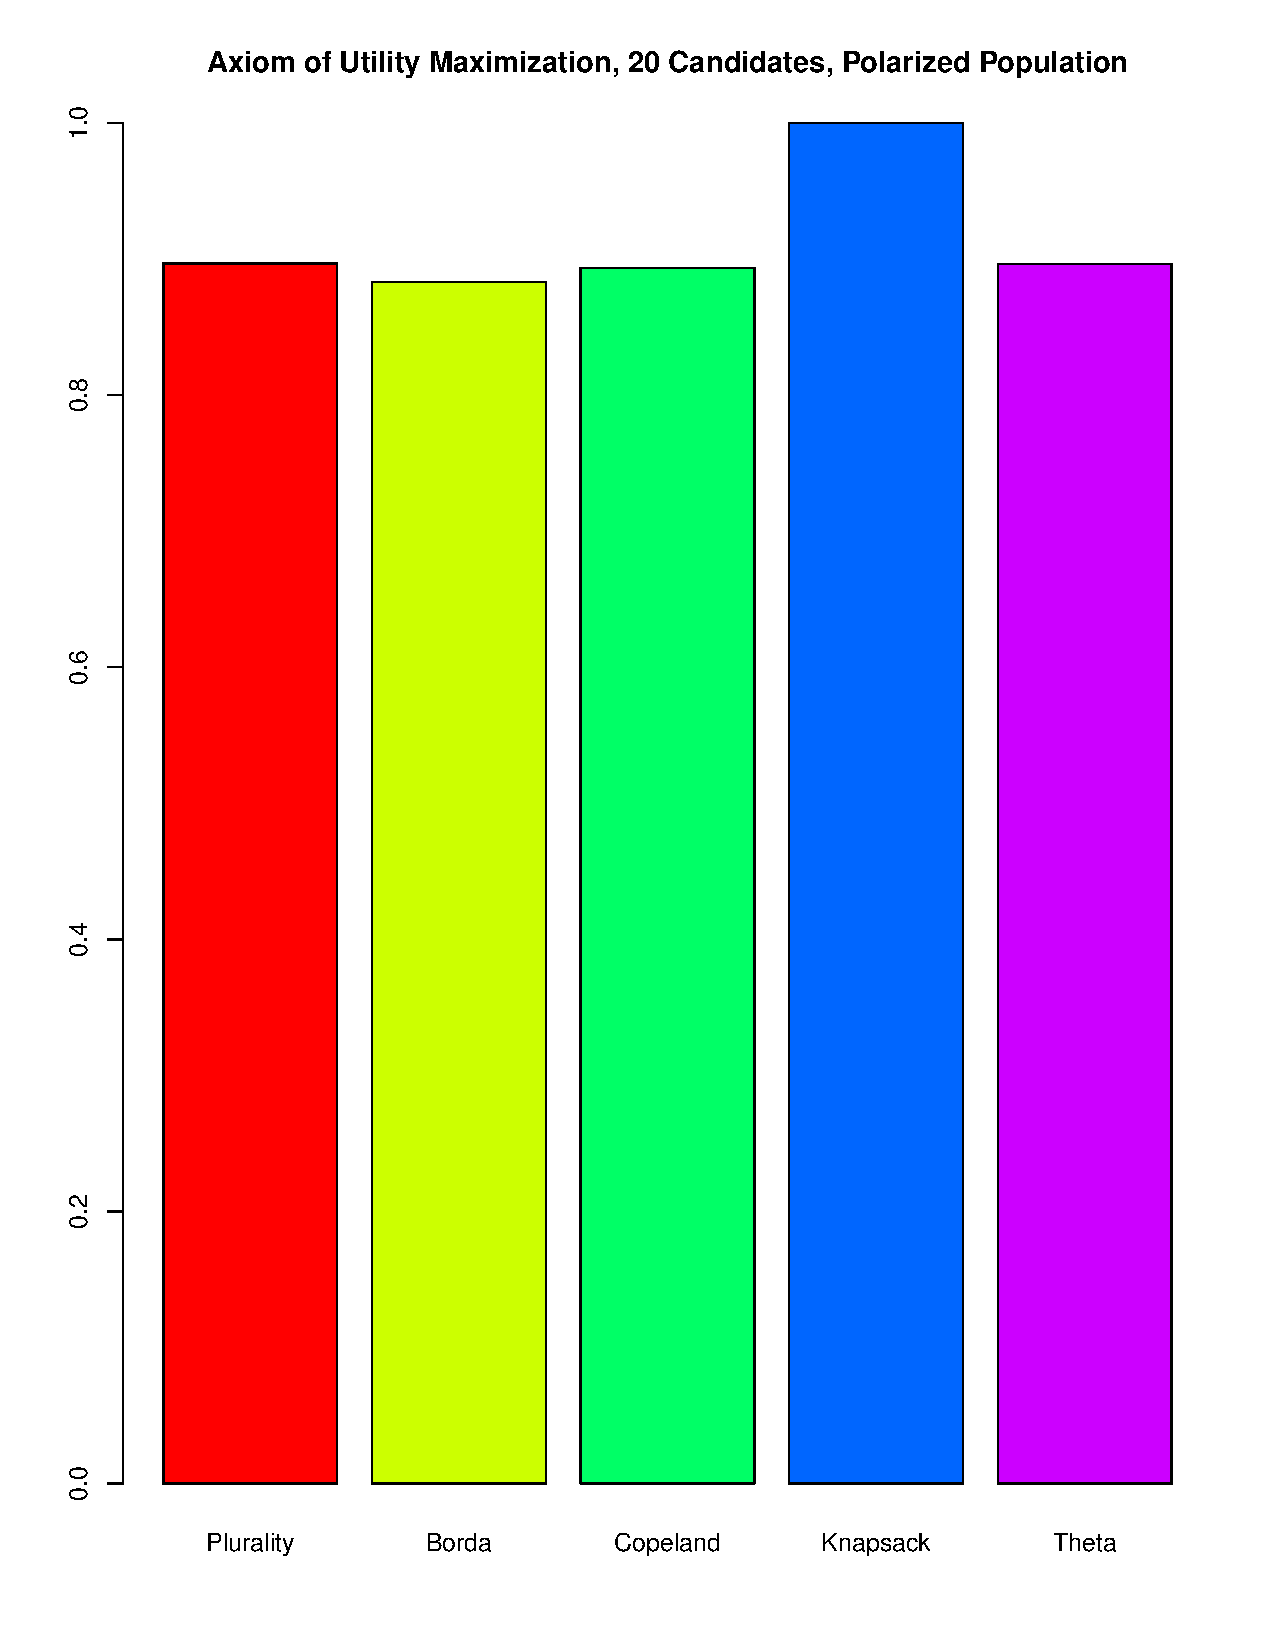
\includegraphics[height=5cm, width=5cm]{Presentation_Plots/Axiom_of_Utility_Maximization_20_Candidates_Polarized_Population.pdf}
           \column{0.58\linewidth}

	 \centering
             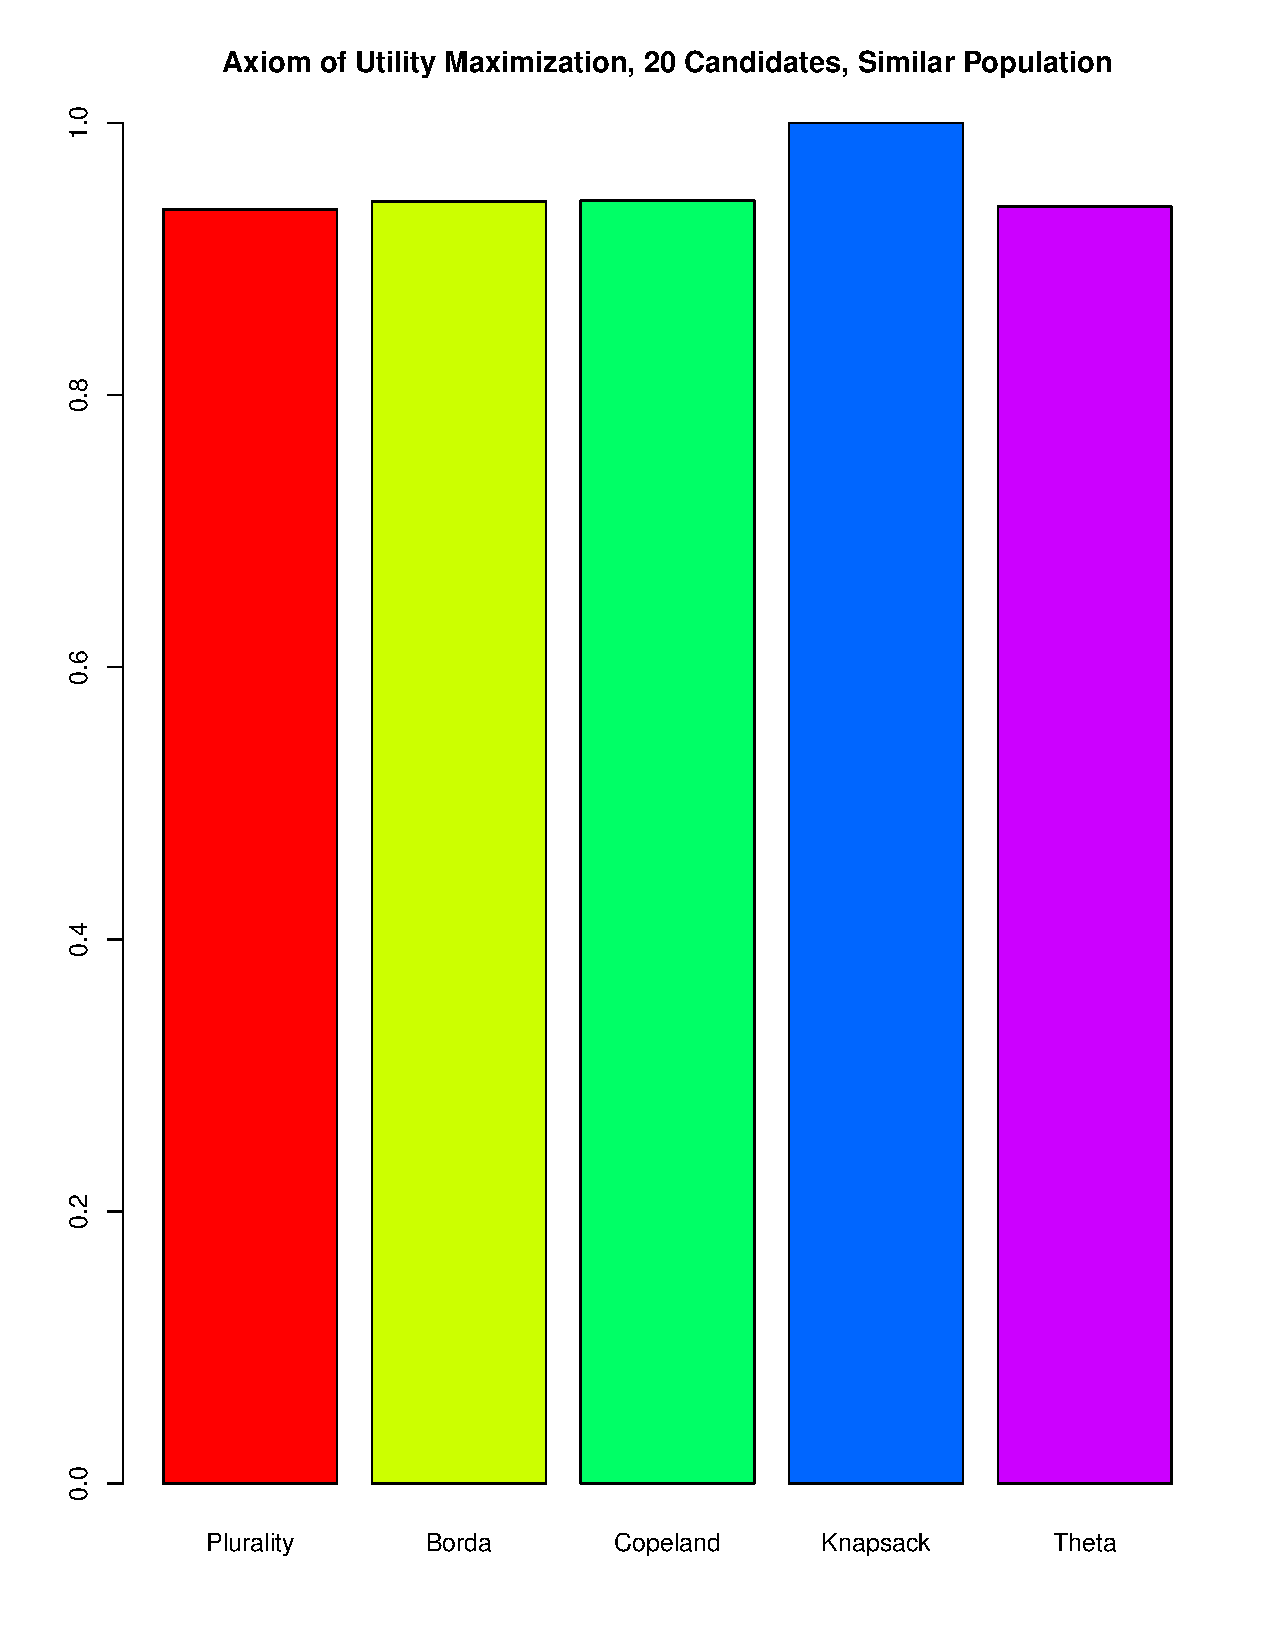
\includegraphics[height=5cm, width=5cm]{Presentation_Plots/Axiom_of_Utility_Maximization_20_Candidates_Similar_Population.pdf}
         \end{columns} 
\end{frame}

\begin{frame}{$\theta$-Minority Consistency}
\begin{columns}
          \column{0.38\linewidth}
             \centering
             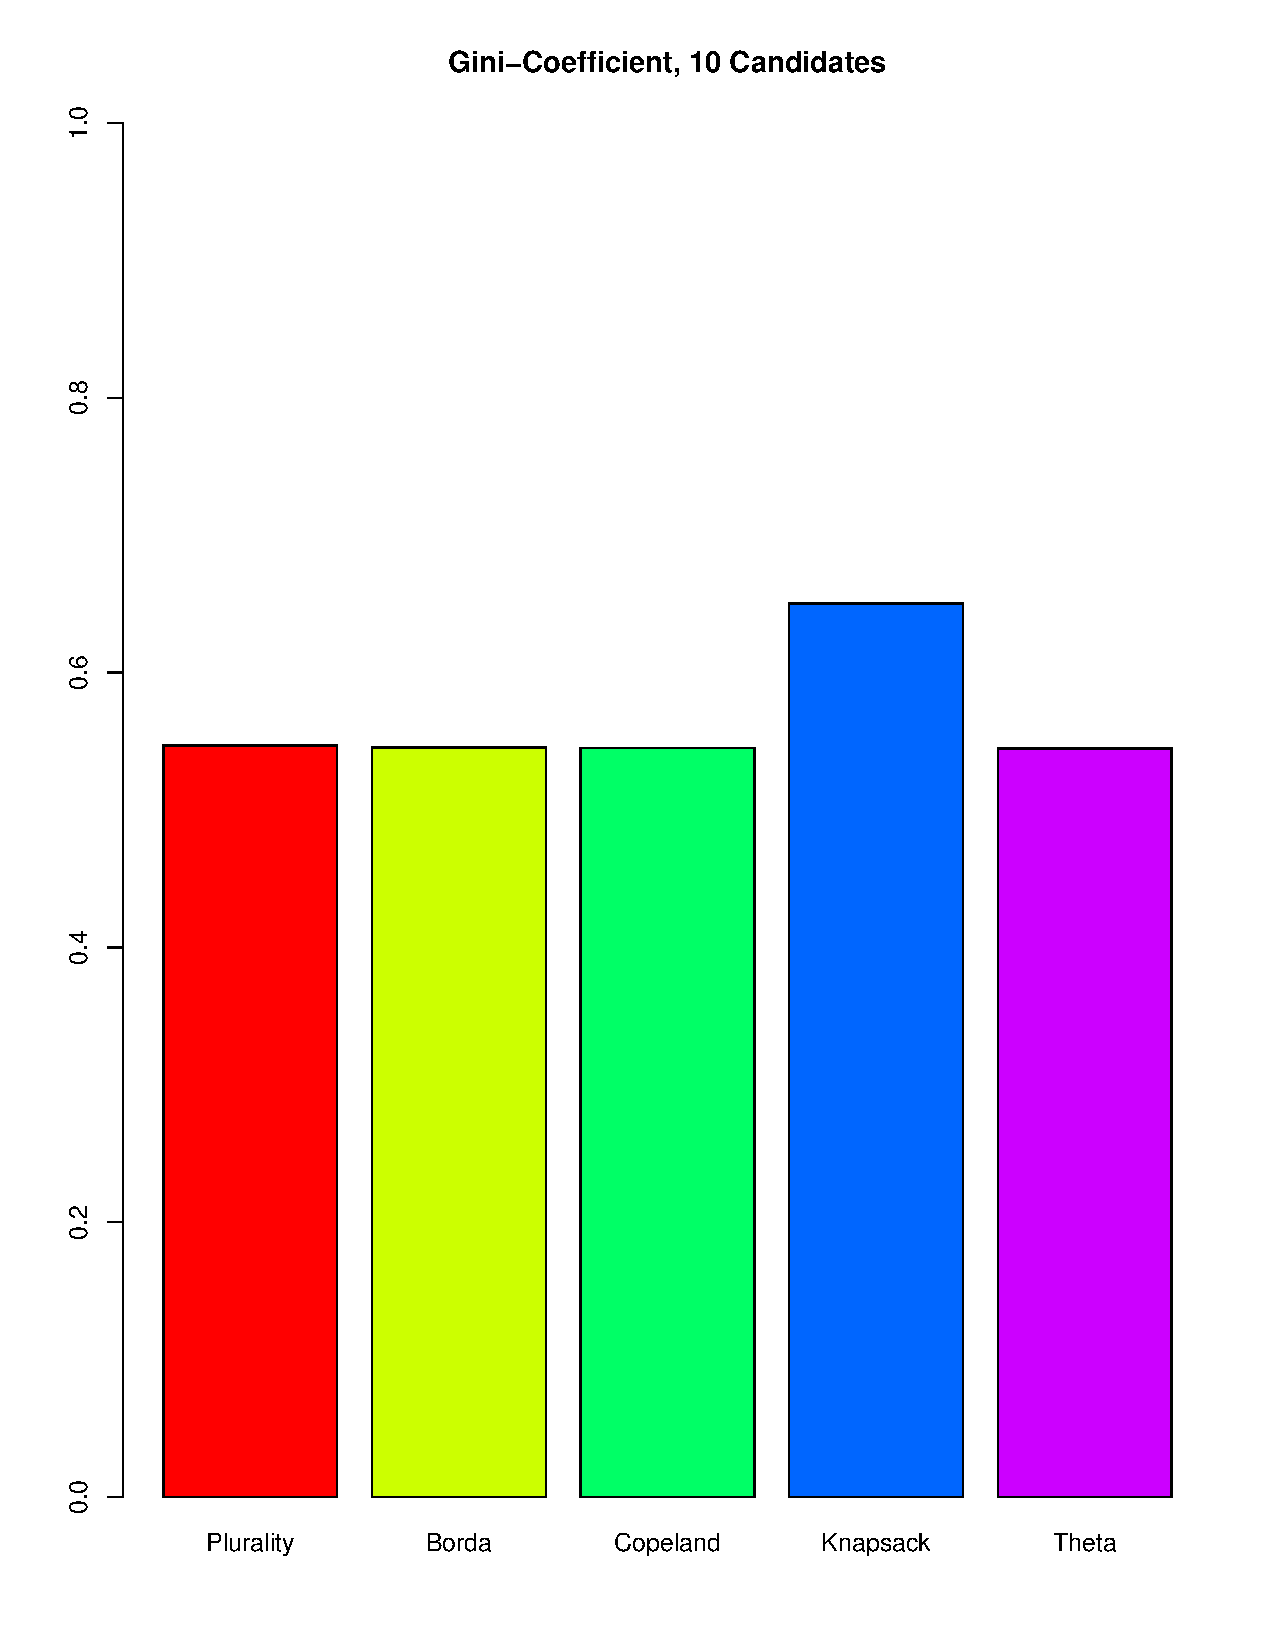
\includegraphics[height=5cm, width=5cm]{Gini_Coefficient_10_Candidates.pdf}
           \column{0.58\linewidth}
             
	 \centering
             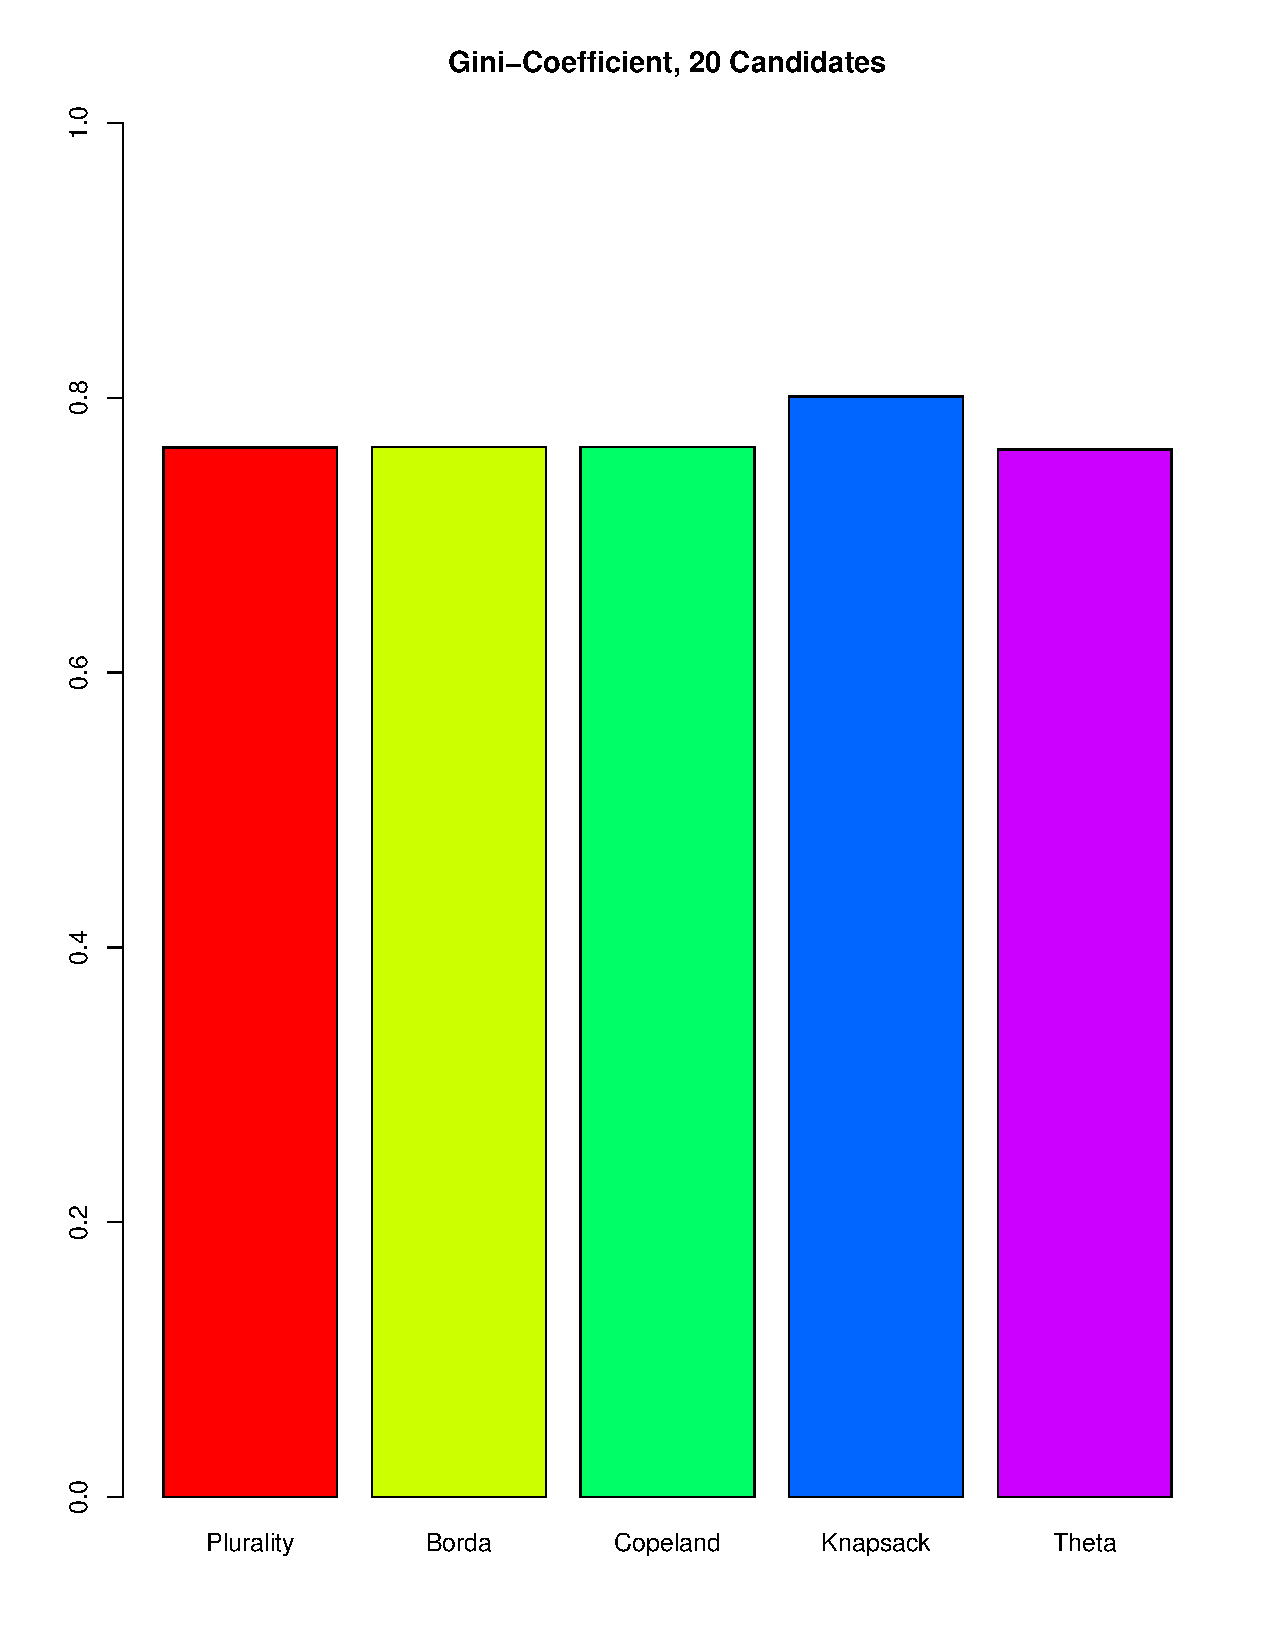
\includegraphics[height=5cm, width=5cm]{Gini_Coefficient_20_Candidates.pdf}
         \end{columns} 
\end{frame}

%\begin{frame}{$\delta$-Equality}
%	\begin{figure}
 %   	\begin{subfigure}
  %      	\includegraphics[]{GINI10}
   %     \end{subfigure}
        
    %    \begin{subfigure}
     %   	\includegraphics[]{GINI20}
      %  \end{subfigure}
       
%\end{frame}
\begin{frame}{Summary of experimental data}
	
\begin{itemize}
\item No rule can be treated as optimal with respect to all desirable properties.
\item The BUM rule deals the best in terms of maximizing utilities on the global level.

\item LGBT rule deals much better in terms of $theta$-Minority Consistency and $\delta$-Equality which concern the equality of users.
\end{itemize}
\end{frame}

\begin{frame}{An Overall Best Rule?}
	
\end{frame}

\begin{frame}{Future Work}

\begin{itemize}
	\item The cost and utility functions could be used to express dependencies (some items form series of articles, cost might vary depending on reader)
	\item Implement slack: in many application leftover budget also has a utility
	\item Find, collect or mine real data (webscraping...).
	\item Build a ready-to-use implementation!
	
\end{itemize}
	
\end{frame}

\begin{frame}{Conclusions}
\begin{enumerate}
	\item \textbf{Overview:} We presented a formal Social Choice framework to give a recommendation of news items.
	\item \textbf{Desirable Properties of Recommendation Sets:} We adjusted multiwinner axioms and devised further desirable criteria: a measure of minority influence, utility maximization and utility equality.
	\item \textbf{Budgeted Voting Rules:} We devised new rules and extended three multiwinner voting rules.
	\item \textbf{Methods:} We proved axiomatic results and ran simulations.
	\item \textbf{Results:}
\begin{itemize}
\item There is a trade-off between maximizing utility and equal utility distribution.
\item The LGBT-Rule favours minority groups, while BUM leads to maximal total utility.
\item In polarized populations, minority groups tend to fare worse and maximal total utility is sub-optimal.
\item More news-items tend to increase utility inequality.
\end{itemize}
\end{enumerate}
\end{frame}

%\bibliography{references}
%\bibliographystyle{plainnat}
%\nobibliography{references}


%\bibliography{references}
\end{document}
